%%%%%%%%%%%%%%%%%%%%%%%%%%%%%%%%%%%%%%%%%%%%%%%%%%%%%%%%%%%%%%%%%
%  _____       ______   ____									%
% |_   _|     |  ____|/ ____|  Institute of Embedded Systems	%
%   | |  _ __ | |__  | (___    Wireless Group					%
%   | | | '_ \|  __|  \___ \   Zuercher Hochschule Winterthur	%
%  _| |_| | | | |____ ____) |  (University of Applied Sciences)	%
% |_____|_| |_|______|_____/   8401 Winterthur, Switzerland		%
%																%
%%%%%%%%%%%%%%%%%%%%%%%%%%%%%%%%%%%%%%%%%%%%%%%%%%%%%%%%%%%%%%%%%

\chapter{Glitches}\label{chap.glitch}

\section{Glitche in der Digitalen Signalverarbeitung}\label{sect.glitch_def}
In der Digitalen Signalverarbeitung ist glitch ein bekannter Fehler, den William I. Fletscher folgendermassen beschreibt: ''Als \textit{glitch}  wird eine ungewollte, flüchtige ''Signalspitze'' bezeichnet, die Zähler aufwärts zählt, Register löscht oder einen ungewollten Prozess startet.'' \cite{F_glitches} \\


Abbildung \ref{fig.glitch.def} zeigt zwei \textit{glitches} in einem Ausgangssignal.\\

\begin{figure}[H]
	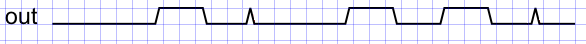
\includegraphics[width=\textwidth]{images/glitch/def_glitch_1.png}
	\caption{Zwei Glitches im Ausgangssignal}
	\label{fig.glitch.def}
\end{figure}


\section{Ursache für Glitches}\label{sect.glitch_ursache}
Der Auslöser sind ungleichzeitig eintreffende Signale, die durch \\
1.) unterschiedlich lange Signalpfade, \\
2.) unterschiedliche Durchlaufverzögerungen der vorangehenden Flip-Flops oder \\
3.) unterschiedliche Logik-Zeiten \\
entstehen, und die in ein \textbf{asynchrones} Bauteil geführt werden. Der Dekoder im asynchronen Bauteil entschlüsselt dadurch kurzfristig einen falschen Wert. \\

Abbilung \ref{fig.glitch.bild1} zeigt ein leicht verzögertes (getaktetes) enable-Signal zu einem anders verzögerten (getakteten) Flip-Flop-Eingangssignal Q. Der Ausgang des Flip-Flops weist kurzzeitig Glitches auf. \\
\begin{figure}[H]
	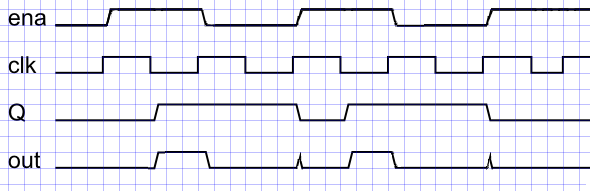
\includegraphics[width=0.8\textwidth]{images/glitch/def_glitch_3.png}
	\caption{Asynchrone Eingangssignale führen zu Glitches}
	\label{fig.glitch.bild1}
\end{figure}


\newpage
\section{Glitches durch Pfadverzögerung}\label{sect.glitch_detect}


\subsubsection{Konzept}
Ein asynchroner Zähler erhält verzögerte Bitwerte. Zählt man binär auf 15, so kann sich beim Übergang von der Zahl 11 zu 12, die falsche Zahl 15, ergeben, sofern die zwei höheren Bits der Zahl 11 verzögert ankommen (siehe Abbildung \ref {fig.glitch.binaer_zahlen}).

\begin{figure}[H]
	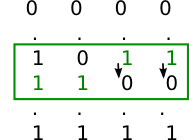
\includegraphics[width=0.3\textwidth]{images/glitch/konzept_verzoegerung.png}
	\caption{Binärwerte des asynchronen Zählers}
	\label{fig.glitch.binaer_zahlen}
\end{figure}

Die Verzögerung der zwei Bits, wird über Routing umgesetzt. 



\subsubsection{Implementation} 
Die Hardware ist das altera board De2 mit dem FPGA Cyclone II. Kompiliert wird das Projekt mit Quartus 13.0sp, der ältsten Quartus-Version, die den Cyclone II unterstützt.

Die Pfad\textit{verlängerung} wird über das Routing über die GPIO-Pins des Headers 1 gemacht (siehe Abbildung \ref{fig.glitch.GPIO}. Dekodiert die asynchrone Logik die Zahl 15, wird das  Reset-Signal an den Zähler gesendet und der Zähler beginnt wieder von 0 an zu zählen. Produziert der Dekoder zur falschen Zeit einen Reset, so ist dies eine Fehlkodierung: ein \textit{glitch}.\\

Das RTL-Diagramm des asynchronen Zählers sieht wiefolgt aus:
\begin{figure}[H]
	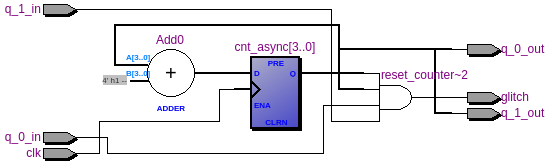
\includegraphics[width=1\textwidth]{images/glitch/RTL_asynchron.png}
	\caption{Asynchroner Zähler mit Routing erzeugt Glitch}
	\label{fig.glitch.RTL_nurGlitch}
\end{figure}

Um die Lösung gegen \textit{glitches} aufzuzeigen, wird dem asynchronen Zähler zur Synchronisation ein Flip-Flop nachgeschalten. Dadurch werden die asychronen Zustände übersehen. 
\begin{figure}[H]
	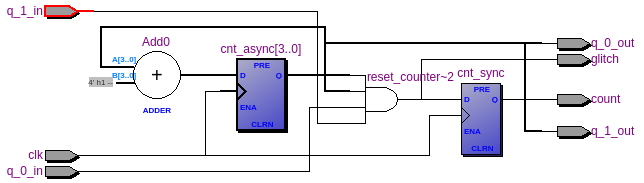
\includegraphics[width=\textwidth]{images/glitch/glitch_asynch_new.png}
	\caption{Glitch-Zähler und synchroner Zähler dazu}
	\label{fig.glitch.RTL_mit_synchr.Zaehler}
\end{figure}

Die Reset-Signale des asynchronen Zählers wie die des synchronisierten Zählers werden an die GPIO Headers ausgegeben, ebenso der Systemtakt.In der Abbildung \ref{fig.glitch.GPIO}) wird das Signal des asynchronen Zählers als Glitch und das Signal des synchronisierten Zählers als Count benannt. In der GPIO-Pinbelegung sieht man auch die Nutzung der zwei oberen Pin-Reihen für das Routing (benannt mit Routing OUT, IN). Der Systemtakt wird als CLK ausgegeben.
\begin{figure}[H]
	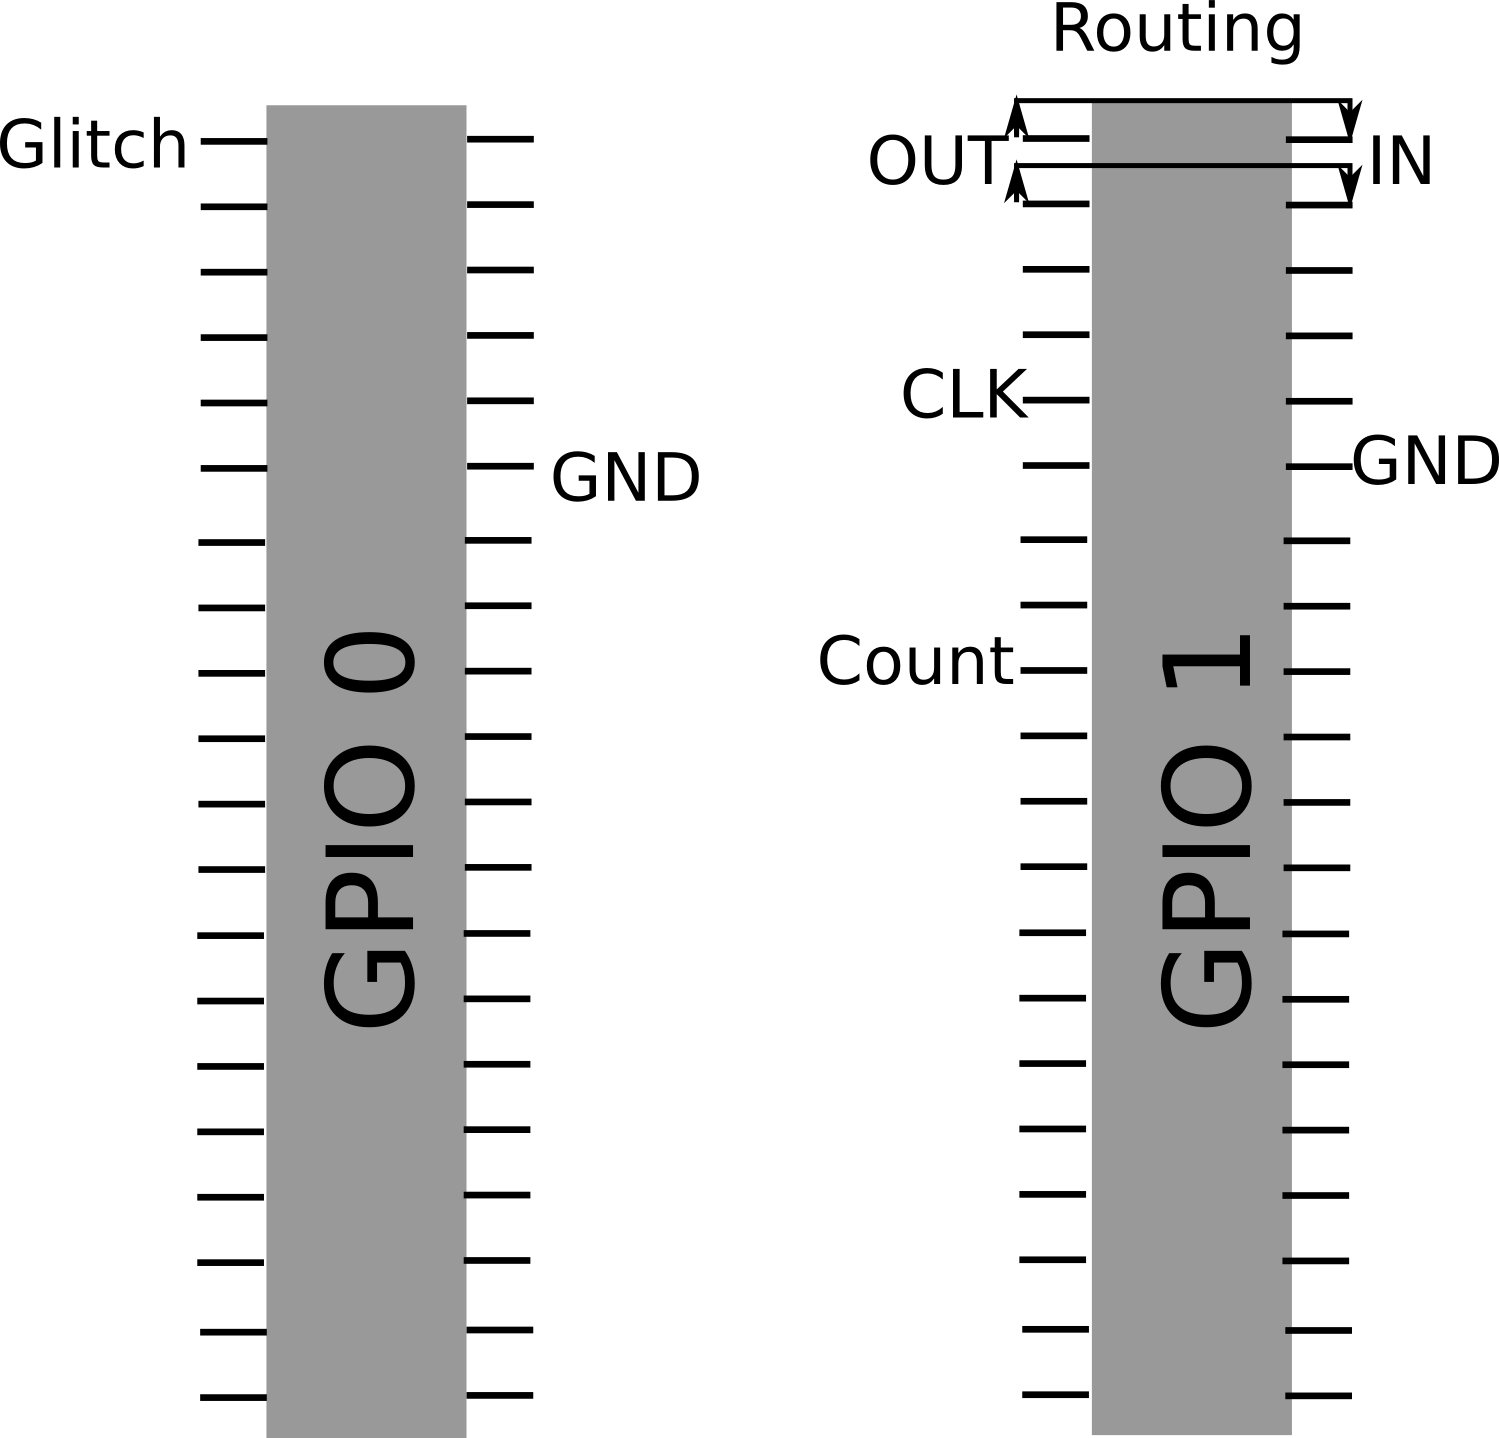
\includegraphics[width=0.5\textwidth]{images/glitch/GPIO_Belegung.png}
	\caption{GPIO Anschlüsse}
	\label{fig.glitch.GPIO}
\end{figure}


\newpage
\section{Resultat }\label{sect.glitch_resultat}

Der Reset des asynchronen Zählers (CH 1), der synchronisierte Reset (CH 2) und der Systemtakt (CH 3) werden am KO ausgegeben. Durch die Synchronisation wird der Wert um 1 Periode (= 20 ns) verzögert.

\begin{figure}[H]
	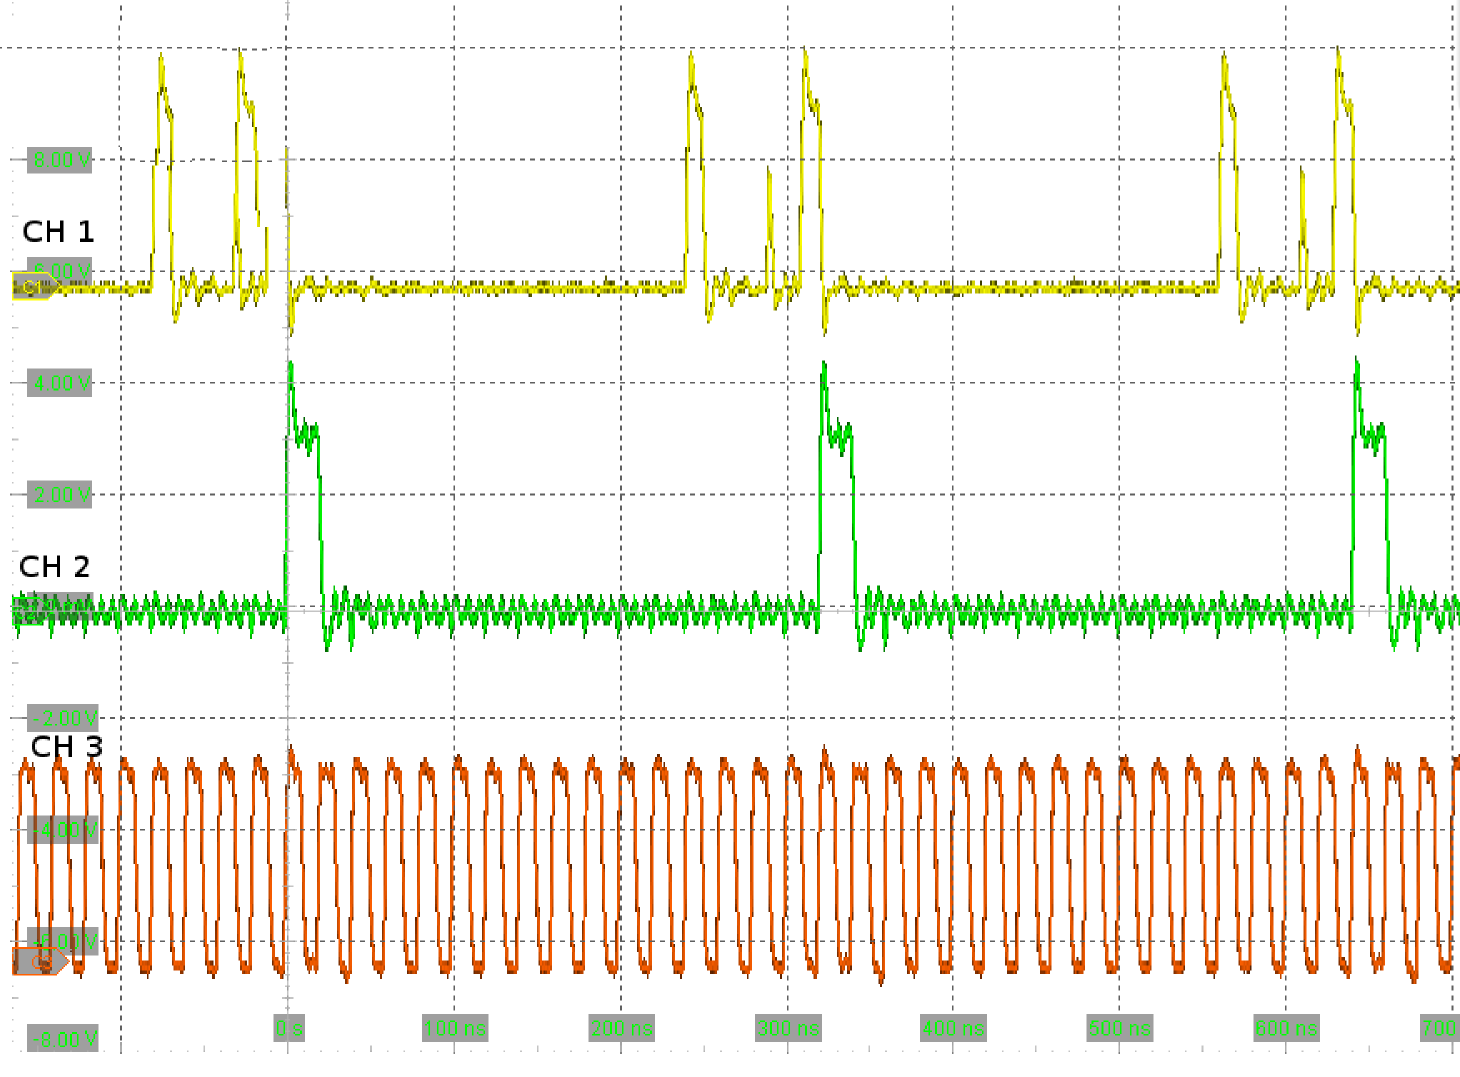
\includegraphics[width=0.6\textwidth]{images/glitch/Glitch_2_good.png}
	\caption{Glitch (gelb), Zähler (grün) und Takt (orange)}
	\label{fig.glitch.result_1}
\end{figure}

 Das \textit{glitch} trifft in der im Übergang von der 11 zur 12 Periode ( = 240 ns ) regelmässig auf. Dies ist das zu erwartende Ergebnis. Ein kurzzeitiges asynchrones Verhalten findet sich auch im Übergang von der 13 zur 14 Periode. Dies ist wenn der binäre Wert 1101 auf 1101 wechselt. Da die zwei niederwertigen Bits verzögert sind, ist das dekodierten des Wertes 1111 plausibel.\\
\begin{figure}[H]
	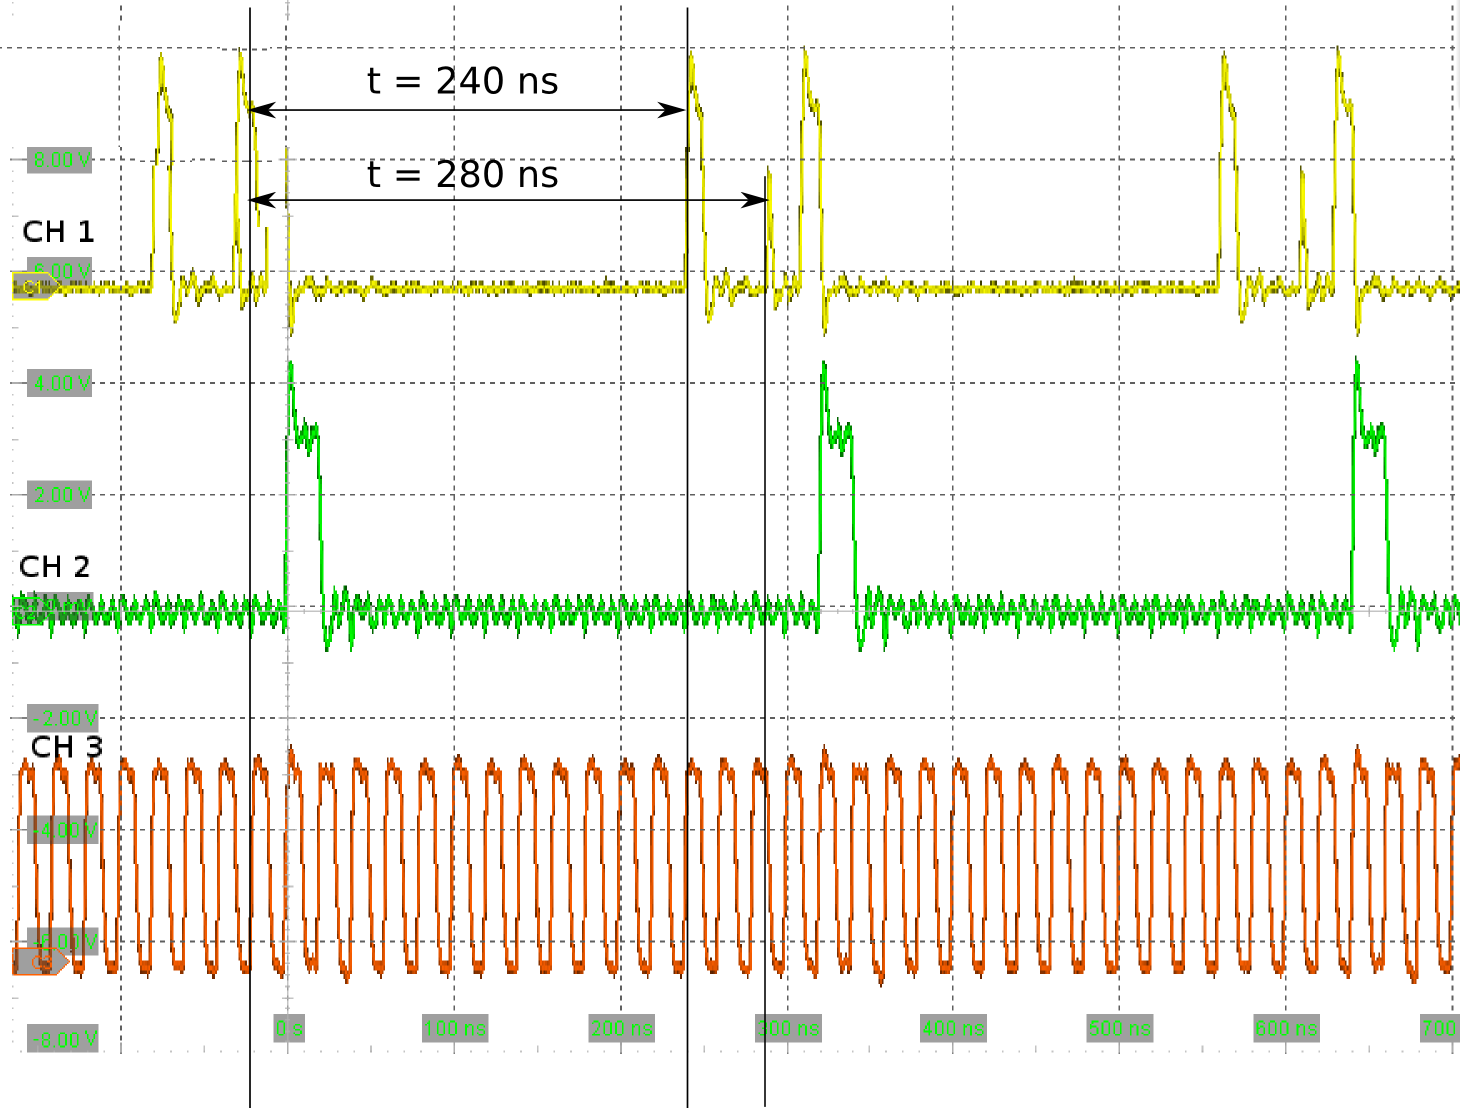
\includegraphics[width=0.6\textwidth]{images/glitch/Glitch_2_timing.png}
	\caption{Zeitanalyse Glitches}
	\label{fig.glitch.result_2}
\end{figure}



